\documentclass[a4paper, 11pt]{article}
\usepackage[utf8]{inputenc}
\usepackage[T1]{fontenc}
\usepackage[polish]{babel}
\usepackage[nofoot,hdivide={2cm,*,1cm},vdivide={1cm,*,1cm}]{geometry}
\usepackage{amsmath, amsfonts}
\usepackage{graphicx}
\graphicspath{ {.} }

\author{Joanna Stachowicz}
\title{Sprawozdanie ze sprawdzianu}
\date{\today}

\begin{document}
\maketitle

\section*{Zadanie 1}
\begin{itemize}
    \item $ \rho\frac{D\textbf{u}}{Dt} = \rho \big( \frac{\partial
    \textbf{u}}{\partial t} + \textbf{u} \cdot \nabla \textbf{u}\big) = -\nabla \overline p + \nabla 
    \cdot \big\{\mu \big(\nabla \textbf{u} + (\nabla \textbf{u})^T - \frac{2}{3}(\nabla \cdot\textbf{u}      
    \big) \textbf{I} \big)\big\} + \rho\textbf{g} $
    
    \item $ \tilde{f}(\xi) = \int^\infty_{-\infty} f(x) e^{-2\pi ix\xi}dx $
    
    \item $ \mathbb{P}\big(\hat{X_n} - z_{1-\frac{\alpha}{2}} \frac{\sigma}{\sqrt{n}} \leq \mathbb{E} X
    \leq \hat{X_n} + z_{1-\frac{\alpha}{2}} \frac{\sigma}{\sqrt{n}}\big) \approx 1 - \alpha $
    
    \item $ \begin{bmatrix} 1 & 2 \\ 3 & 4 \end{bmatrix} \otimes \begin{bmatrix} 0 & 5 \\ 6 & 7 \end{bmatrix} =
    \begin{bmatrix} 1 \begin{bmatrix} 0 & 5 \\ 6 & 7 \end{bmatrix} & 2 \begin{bmatrix} 0 & 5 \\ 6 & 7 \end{bmatrix} \\
    3 \begin{bmatrix} 0 & 5 \\ 6 & 7 \end{bmatrix} & 4 \begin{bmatrix} 0 & 5 \\ 6 & 7 \end{bmatrix} \end{bmatrix} $
    
\end{itemize}

\section*{Zadanie 2}

\subsection*{a) Generowanie kluczy SSH}
\begin{itemize}

\item komendą \verb+ssh-keygen -t rsa+ generuję sobie parę kluczy - prywatny i publiczny.
\item flaga \textsf{t} służy do określenia typu klucza, w powyższym przypadku to \textsf{rsa}
\item Zrzut ekranu terminalu po wygenerowaniu klucza:




\noindent
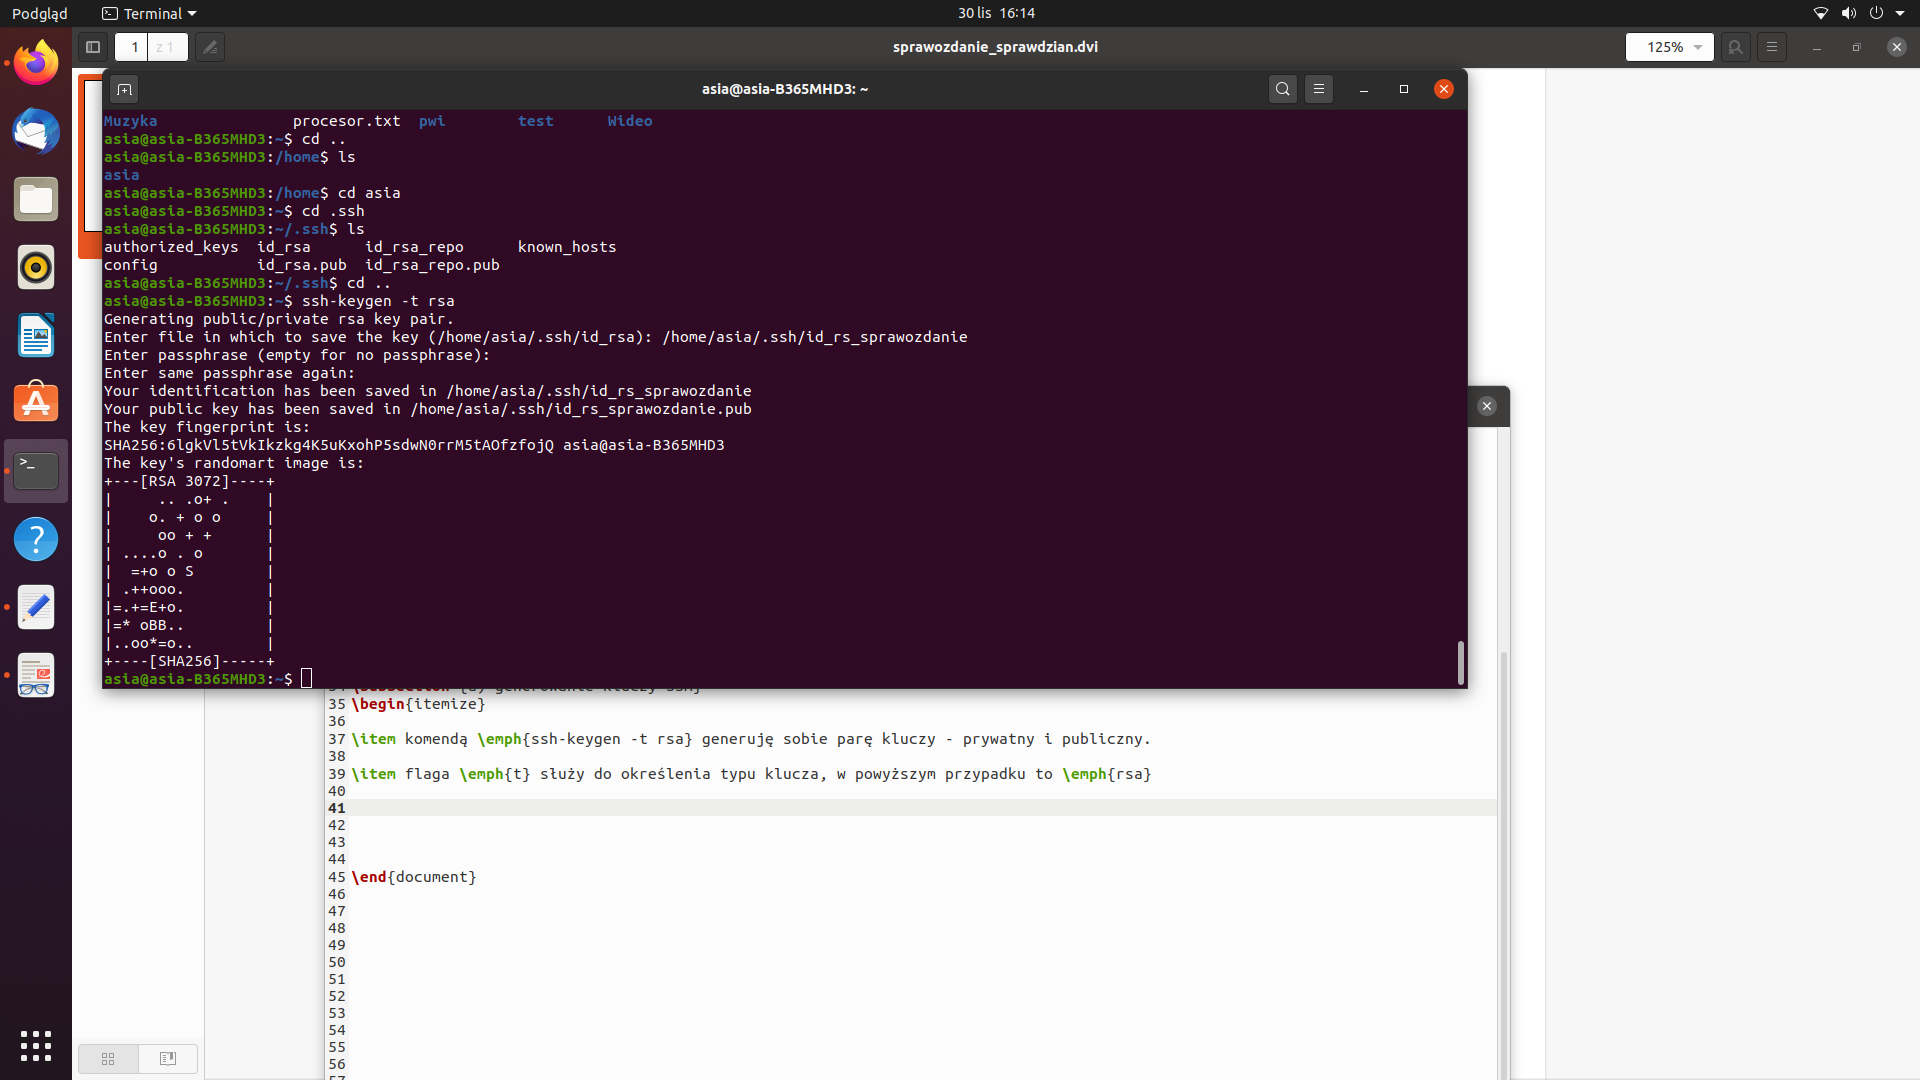
\includegraphics[scale = 0.2]{screen_ssh-keygen.png}

\item Powyższą operację powtarzam dwókrotnie, w celu wygenerowania dwóch par kluczy ---do serwera i repozytorium.

\end{itemize}
\newpage
\subsection*{b) Przeniesienie klucza na zdalny serwer}
\begin{itemize}

\item łączę się ze zdalnym serwerem przy pomocy polecenia \verb+ssh s324807@pwi.ii.uni.wroc.pl+
\item kopiuję klucz na serwer za pomocą polecenia:

\verb+ssh-copy-id -i ~/.ssh/id_rs_sprawozdanie s324807@pwi.ii.uni.wroc.pl+

\item flaga \textsf{i} wskazuje ścieżkę do pliku, w którym znajduje się klucz
\item \textsf{s324807} to nazwa mojego użytkownika 
\item \textsf{pwi.ii.uni.wroc.pl} to domena serwera


\end{itemize}

\subsection*{c) Utworzenie pustego repozytorium}
\begin{itemize}

\item Loguję się na moje konto na GitHubie
\item Na swoim profilu wyszukuję:
\begin{itemize}

\item {\bf Repositories}
\item {\bf New}
\item {\bf Repository name}
\item {\bf Create repository}

\end{itemize}

\item dodaję klucz na repozytorium
\begin{itemize}

\item wchodzę w utworzone przed momentem repozytorium 
\item wybieram {\bf Settings}
\item {\bf Deploy keys}
\item dodaję swój klucz PUBLICZNY do repozytorium

\end{itemize}
\end{itemize}

\subsection*{d) Tworzenie pliku konfiguracyjnego}
\begin{itemize}
\item \textsf{Host} to nazwa, którą będziemy stosować do zalogowania się na serwer, czyli \textsf{pwi-sprawdzian}
\item \textsf{HostName} to domena hosta, z którym chcę się łączyć, więc wpisuję \verb+pwi.ii.uni.wroc.pl+
\item \textsf{User} to nazwa użytkownika, z którego będę się łączyć do serweru, czyli \verb+s324807+
\item \textsf{IdentityFile} to ścieżka pliku do klucza PRYWATNEGO 
\item Poniżej screen z terminala z edycji pliku config w edytorze nano:


\noindent
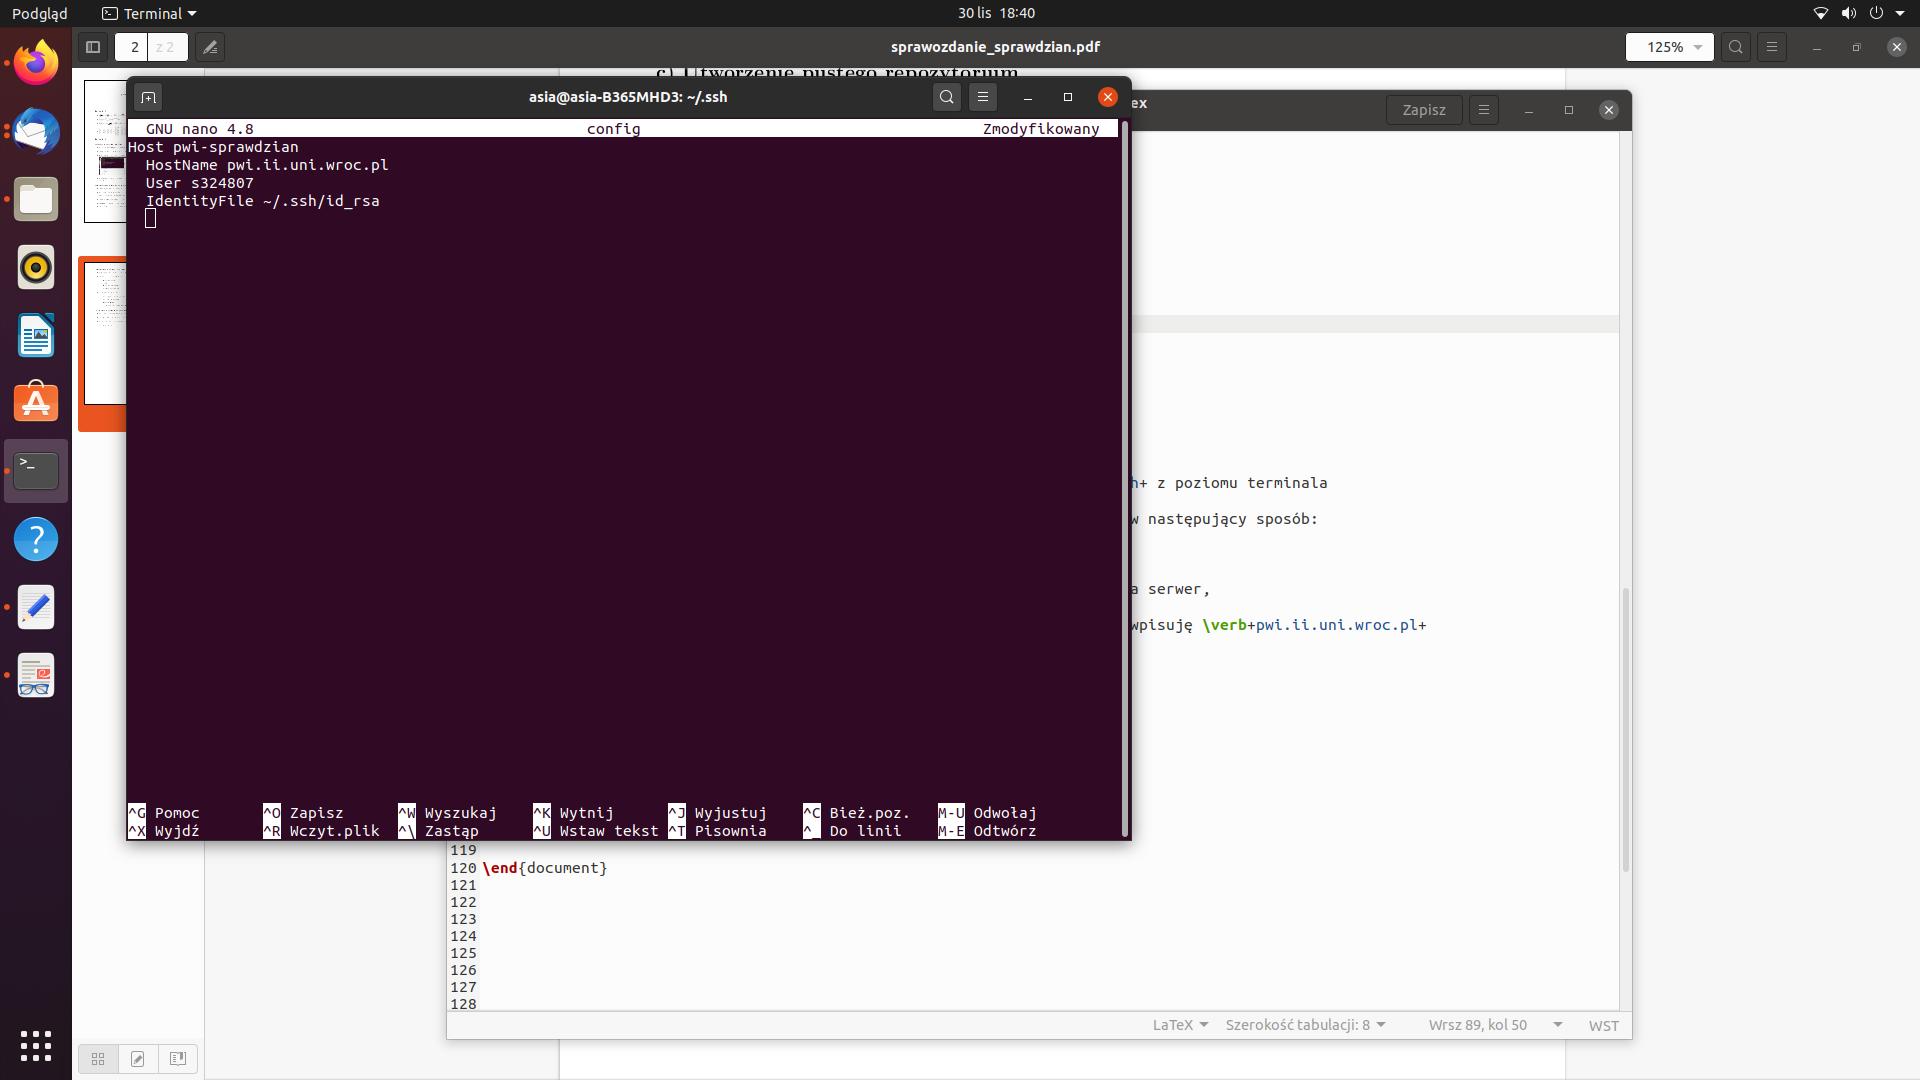
\includegraphics[scale = 0.2]{edit_config.png}
\end{itemize}


\subsection*{e) Przekierowanie klucza lokalnego}

do pliku konfiguracyjnego \textsf{config} należy dopisać \textsf{ForwardAgent yes}, żeby uruchomić agenta ssh

\section*{Zadanie 3}

\subsection*{a) Klonowanie repozytorium i forwardowanie klucza}

\begin{itemize}
\item dodaję mój klucz do ssh agenta poleceniem \verb+ssh-add ~/.ssh/id_rsa+
\item \verb+~/.ssh/id_rsa+ to ścieżka do pliku z kluczem, który chcę przeforwardować
\item Nie powinno się generować nowego klucza na zdalnym serwerze, ponieważ narażałoby to na\\ niebezpieczeństwo 
wrażliwe dane (dzięki kluczowi prywatnemu), do których dostęp mogliby mieć inni\\ użytkownicy serwera, 
stąd określenie "\emph{brzydkie} rozwiązanie"
\item loguję się na serwerze za pomocą polecenia \verb+ssh pwi-sprawdzian+
\item klonuję repozytorium poleceniem

\verb+git clone git@github.com:JoannaStachowicz/PWI-sprawdzian-s324807.git+
\end{itemize}

\subsection*{(b) Pobieranie pliku i komitowanie zmian}
\begin{itemize}
\item wchodzę do katalogu ze sklonowanym repozytorium komendą \verb+cd PWI-sprawdzian-s324807+
\item pobieram plik poleceniem \verb+wget http://www.ii.uni.wroc.pl/~lisu/zadanie.tar.gz+
\item rozpakowuję plik komendą \verb+tar -xf zadanie.tar.gz+, gdzie:
\begin{itemize}
\item flaga \textsf{x} wskazuje, że plik ma być rozpakowany w archiwum
\item flaga \textsf{f} wskazuje plik który ma zostać rozpakowany 
\end{itemize}
\item Zmieniam status plików na śledzone a następnie commituję zmiany nastepującymi poleceniami:
\begin{itemize}
\item \verb+git add+
\item \verb+git commit+
\end{itemize}
\end{itemize}

\subsection*{c) Wyliczenie funkcji}
\begin{itemize}
\item wyliczam funkcję skrótu {\bf MD5} ze stringa {\bf s324807} za pomocą polecenia:

\verb+echo -n s324807 | md5sum+
\item szukam otrzymanego folderu komendą:
\verb+find -type d -name "b5a4c4b7b541173e1fe33f16b205cd65"+
\begin{itemize}
\item \textsf{type -d}, ponieważ szukamy folderu
\item \textsf{name} nazwa poszukiwanego przez nas folderu 
\end{itemize}
\item {\bf Rozwiązanie zadania 1}:
\begin{itemize}
\item Szukam użytkowników spotify z Polski za pomocą komendy

\verb+grep -xc "[a-zA-Z@.:0-9]* | Country = POLAND .*" users.db+
\item flaga \textsf{x} odpowiada za szukanie wyrażenia w całym wersie
\item flaga \textsf{c} zlicza wystąpienia poszukiwanego wyrażenia w podanym pliku 
\item Żeby uzyskać procentowy stotunek, wyliczam wszystkich użytkowników, którym ukradziono hasła, komendą:
\verb+grep -xc ".*" users.db+
\item Używam Pythona jako kalkulatora i wyliczam stosunek procentowy.\\
{\bf Wynik:} \verb+1.3893032175580652 %+
\end{itemize}
\newpage
\item {\bf Rozwiązanie zadania 2}
\begin{itemize}
\item Przy pomocy polecenia \verb+sed 's/[^:]*://' users.db > pomocniczy.txt+ usuwam wszystko od początku wersu, do hasła 
\item Tworzę poleceniem \verb+touch passwords.txt+ plik, o którym mowa w zadaniu
\item Z pliku pomocniczego usuwam pozostałe znaki następujące po hasłach, a rezultat zapisuję w pliku {\bf passwords.txt}:
\verb+sed 's/ |.*//' pomocniczy.txt > passwords.txt+
\item Teraz w pliku passwords.txt znajdują się wyłącznie hasła użytkowników 
\end{itemize}
\end{itemize}


\begin{thebibliography}{3}
\bibitem{}
 \begin{verbatim}
 http://www.math.uni.wroc.pl/~admor/LaTeX/latex_6.pdf
 \end{verbatim}
\bibitem{}
 \begin{verbatim}
 https://pl.wikipedia.org/wiki/Pomoc:Wzory
 \end{verbatim}

\end{thebibliography}


\end{document}



























